\section{Task Force Arrowhead Radio (TFAR)}
\label{TFAR}
\subsection{Tastaturkürzel}
\begin{longtable}{|p{2cm}|p{5 cm}||p{2cm}|p{4cm}|} 
	\caption[Trupp]{die wichtigsten Tasten TFAR Tasten} \\ 
	\hline
	\cellcolor{backcolor} \textbf{Taste} & \textbf{Beschreibung} & \cellcolor{backcolor}\textbf{Taste} & \textbf{Beschreibung}  \\ 
	\hline
	\cellcolor{backcolor} STRG + P & SR Funkgerät öffnen & \cellcolor{backcolor}  ALT + P &  LR Funkgerät öffnen \\
	\hline
	\cellcolor{backcolor} PTT im TS\footnote{Push to Talk bzw. Spracherkennung im Teamspeak} & direkt sprechen & \cellcolor{backcolor}  Caps Lock & Auf SR Funk funken \\
	 \hline
	\cellcolor{backcolor} T & Aud SR Additional Channel funken & \cellcolor{backcolor}  Y & Auf LR Additional Channel funken \\
	 \hline
	\cellcolor{backcolor} STRG + TAB & Gesprächslautstärke einstellen\footnote{whispering / normal / yelling} & \cellcolor{backcolor}  & \\
	 \hline
	\cellcolor{backcolor} SHIFT + P & Unterwasserfunkgerät & \cellcolor{backcolor}  STRG + \~ & Auf Unterwasserfunk funken \\
	 \hline
\end{longtable}
\subsection{Short Range Funkgerät (AN/PRC – 152)}
	\begin{minipage} [b]{0.5\textwidth}
		\begin{enumerate}
			\item Lautstärke einstellen
			\item aktueller Kanal
			\item aktuelle Funkfrequenz
			\item Stereo Einstellungen\nl (linkes Ohr / rechtes Ohr)
			\item Funkfrequenz festlegen
			\item Frequenz löschen
			\item Frequenz bestätigen
			\item Funkkanal wechseln
			\item Umschaltung zwischen\nl Lautsprecher -- Kopfhörer
			\item Additional Channel festlegen
		\end{enumerate}
	\end{minipage}
	\begin{minipage}[t]{0.4\textwidth}
		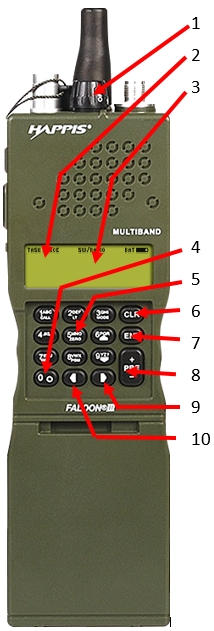
\includegraphics[width=\textwidth]{./img/tutorials/tfar/TFAR_SR_Radio.png}
	\end{minipage}


\subsection{Long Range Funkgerät (RT-15236 (ASIP) - LR)}
\begin{minipage}[t]{1\textwidth}
	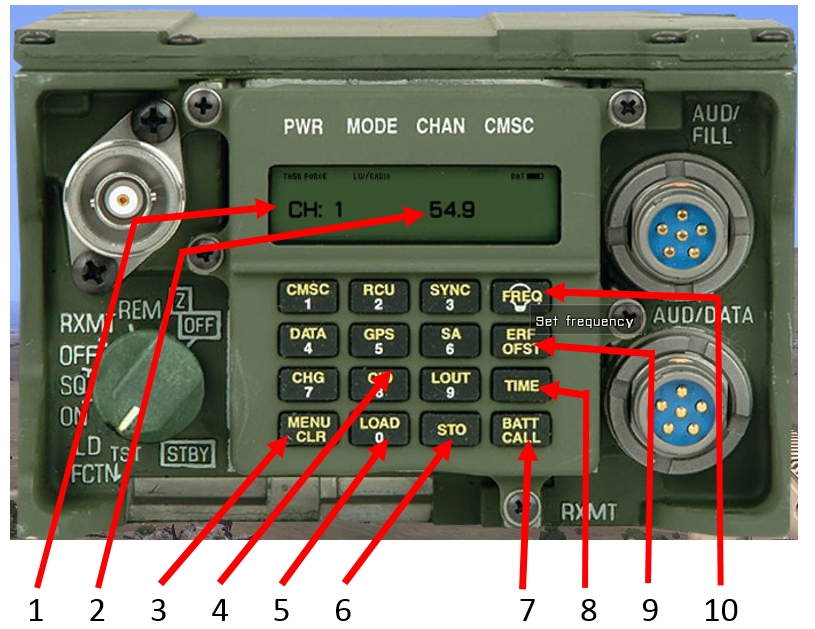
\includegraphics[width=\textwidth]{./img/tutorials/tfar/TFAR_LR_Radio.png}
\end{minipage}
\begin{enumerate}
	\item aktueller Kanal
	\item aktuelle Funkfrequenz
	\item Frequenz löschen
	\item Tastenfeld zur Eingabe der Funkfrequenz
	\item umschalten zwischen Lautsprecher und Kopfhörer
	\item Stereo Einstellungen (linkes Ohr / rechtes Ohr)
	\item Lautstärke  senken
	\item Lautstärke erhöhen
	\item Additional Channel festlegen
	\item Frequenz bestätigen
\end{enumerate}
